% Yiyong Sun,yiyognhit@gmail.com,2017.03.05 %% The current version should be listed at the first sight. Any changes, mark your name mailbox and the date

\documentclass[a4paper]{article}%{report}%{book}
%\newcommand{\CurrentDate}
\usepackage[section]{placeins}
\usepackage{longtable}
\usepackage{float}
\usepackage{url}
\usepackage{CJKutf8}
\usepackage{amsfonts}
\usepackage{amsmath}
\usepackage{mathrsfs}
\usepackage{latexsym}
\usepackage{graphicx}
%\usepackage{exCJK}
%\usepackage[superscript]{cite}
%\usepackage[dvipdfmx,unicode,           %dvi-->pdf ????
            %bookmarksnumbered=true]{hyperref}
%\newtheorem{remark}{注解}

 % {gkai}{gbsn}

\begin{document}
\begin{CJK}{UTF8}{gbsn}
\title{高速高精度光机电一体化技术与设备}
\author{高会军
\thanks{\textbf{哈尔滨工业大学智能控制与系统研究所}}
\date{\CurrentDate} % Curent Date
}
\maketitle
\clearpage
\tableofcontents
\clearpage

\section{表面贴装技术背景及现状}

贴片机是一种高精尖光机电一体化设备,主要用来全自动高精度、高速地贴放电子元器件,是整个表面贴装(Surface mount technoloty,简称SMT)生产线中最复杂、最核心的装备。随着中国电子制造业的高速发展,中国的SMT技术及产业也同步迅猛发展,表面贴装生产线的关键设备——贴片机在中国的保有量已居世界前列,SMT贴片机市场占全球的40\%。目前,中国SMT行业使用的主流中高速泛用贴片机让然处于国外垄断状态,每年进口贴片机的开销达10亿美元以上,而中国自主研发的低速专用贴片机由于产能低下,功能单一,稳定性差等原因,无法胜任大规模高速高精度的贴装任务。因此,国产高速高精度泛用贴片机的研发势在必行。

哈工大智能控制与系统研究所着眼中国SMT行业发展的核心问题,于2010年起,自主研发面向中国市场的中高速泛用贴片机。长江学者高会军教授带领包括教授、副教授、博士生和硕士生等50余人的科研团队长期研究贴片机制造中的重点难点问题。这些研究包括复杂的机械结构设计、高速高精度运动控制系统、稳定可靠的人机交互界面及高效高精度的图形图像算法等。目前,这些技术及方法都得到了有效验证,自主设计的样机将于XXX完成装配。这款贴片机具有完备的自主知识产权,基于该项目已经申请国家专利120余项,授权50项,并申请美国、日本国际专利各1项。已经完成装机测试的贴片机贴装速度可达22000CPH,可保证长时间稳定运行。相比国内其他产品,该款产品机械机构更稳定,运动控制系统定位精度更高,响应速度更快,图形图像算法支持全部种类芯片的识别并且不依赖商业库,软件系统更为可靠及人性化,完整的路径优化算法极大提高了贴装效率。该款产品的出现,填补了国内中高速泛用贴片机的空白,十分有望打破国内贴片机市场长期被国外厂商垄断的局面。科研团队在研制这款贴片机的过程中掌握并使用了多种核心的高精尖工业信息技术,例如多轴伺服系统协同、视觉伺服、分布式软件研发等技术,这些技术能够移植到相关的基础制造业中,实现我国基础制造业独立,实现彻底的中国制造。
%近年来,龙江的信息电子产品制造蓬勃发展,每年都涌现出许多新的贴装生产线,现有的贴装生产线每年也有贴片机更新换代的需求。针对龙江市场的贴片机缺口
\subsection{起源}
对于PIC器件来说,以往普遍采用DIP、PLCC或者SOIC的封装形式。然而,随着人们对紧凑型、高性能产品的需求增加,要求引入更为先进的PIC器件。现如今的闪存器件可以采用SOP、TSOP、VSOP、BGA和微小型BGA封装形式。高性能的微型控制器、CPLD器件和FPGA器件一直到可以采用QFP、BGA和微型BGA封装形式,其所拥有的引脚数量范围从44条一直可以达到超过800条以上。

由于非常多的引脚数量和很小的外形尺寸,这些元器件中的大部分仅能够采用微细间距的封装形式。微细间距的元器件所拥有的引脚非常脆弱,间距只有0.508mm(20 mils)或者说间隙几乎没有。这样人们就将目光瞄向了使用PIC器件来应对这一挑战。 具有高密度和高性能的PIC器件价格是很昂贵的,要求采用高质量的编程设备,需要拥有非常优异的过程控制,以求将元器件的废弃程度降低到最小的程度。

在采用手工编制程序的操作过程中,微细间距元器件实际上肯定会遭遇到来自共面性和其它形式的引脚损伤因素的威胁。如果说引脚受到了损伤的话,那么将可能导致焊接点可靠性出现问题,会提升生产制造过程中的缺陷率。同样,高密度的元器件实际上将花费较长的编程时间,这样就会降低生产的效率。
\subsection{发展过程}
\subsection{表面贴装技术核心问题}
\subsection{前景}
\section{泛用贴片机研究意义}
市场需求大,但是依赖进口。国产低端。核心技术亟待突破。
\section{泛用贴片机的重难点问题}
\subsection{机械结构设计}
\subsubsection{机架}
机架是机器的根底,一切的传动,定位组织均和供料器均结实固定在它上面,因而有必要具有满足的机械强度和刚性。当前贴片机有各种形式的机架,首要包含全体铸造式和钢板烧焊式。第一种全体性强,刚性好,变形微小,作业时安稳,通常应用于高级机;第二种具有加工简略,本钱较低的特点。机器详细选用哪种布局的机架取决于机器的全体描绘和承重,运转进程中应平稳,轻松,无震动感。

\textbf{(1)拱架式}
拱架式(又称动臂式)机器是最传统的贴片机,具有较好的灵活性和精度,适用于大部分原件,高精度机器一般都是这种类型,但其速度无法与复合式、转塔式和大型平行系统相比。不过原件排列越来越集中在源不见伤,比如有引线的四边扁平封装器件(Quad flat package, QFP)和球栅阵列器件(Ball grid array, BGA),安装精度对高产量有至关重要的作用,复合式、转塔式和大型平行系统一般不适用于这种类型的原件安装。拱架式机器分为单臂式和多臂式,单臂式是最早发展起来的现在仍然使用的多功能贴片机。在单臂式基础上发展起来的多臂式贴片机可将工作效率成倍提高,例如美国Universal公司的GSM2贴片机就有两个动臂安装头,可分别交替对凉快PCB同时进行安装,拱架式机器的结构图如图\ref{fig301}所示。
\begin{figure}[htb!]
\centering
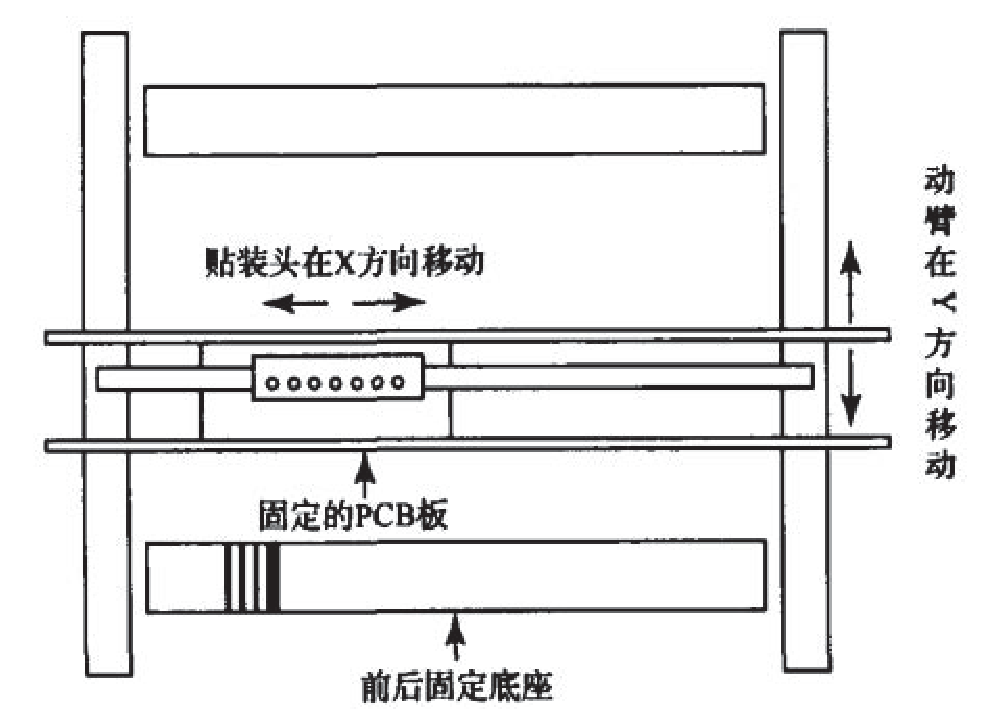
\includegraphics[width=0.6\textwidth]{fig301.eps}
\caption{拱架式机器结构图}
\label{fig301}
\end{figure}

在拱架式结构中,元件送料器、基板(PCB)是固定的,贴片头(安装多个真空吸料嘴)在送料器与基板之间来回移动,将元件从送料器取出,经过对元件位置与方向的调整,然后贴放于基板上。由于贴片头是安装于拱架型的X/Y坐标移动横梁上,所以得名。

拱架型贴片机对元件位置与方向的调整方法:

1)机械对中调整位置、吸嘴旋转调整方向。

2)激光识别、X/Y坐标系统调整位置、吸嘴旋转调整方向,这种方法可实现飞行过程中的识别,但不能用于球栅列陈元件BGA。

3)相机识别、X/Y坐标系统调整位置、吸嘴旋转调整方向,一般相机固定,贴片头飞行划过相机上空,进行成像识别,比激光识别耽误一点时间,但可识别任何元件,也有实现飞行过程中的识别的相机识别系统,机械结构方面有其它牺牲。

这种形式由于贴片头来回移动的距离长,所以速度受到限制。一般采用多个真空吸料嘴同时取料(多达上十个)和采用双梁系统来提高速度,即一个梁上的贴片头在取料的同时,另一个梁上的贴片头贴放元件,速度几乎比单梁系统快一倍。但是实际应用中,同时取料的条件较难达到,而且不同类型的元件需要换用不同的真空吸料嘴,换吸料嘴有时间上的延误。

这类机型的优势在于:系统结构简单,可实现高精度,适于各种大小、形状的元件,甚至异型元件,送料器有带状、管状、托盘形式。适于中小批量生产,也可多台机组合用于大批量生产。

\textbf{(2)复合式}

复合式机器是从拱架式机器发展而来,它集合了转塔式和拱架式的特点,在动臂上安装有转盘,像Siemens的Siplace80S25贴片机,有两个带有12个吸嘴的旋转头,如图\ref{fig302}所示。Universal公司也推出了带有30个吸嘴的旋转头,称之为“闪电头”,两个这样的旋转头安装在Genesis贴片机平台上,可以实现每小时60000片贴片速度。从严格意义上来说,复合式机器仍属于动臂式结构。由于复合式机器可通过动臂数量来提高速度,具有较大灵活性,因此它的发展前景被看好,例如Sienmens推出的HS60机器就安装有4个旋转头(如图\ref{fig303}),贴装速度可达每小时60000片。
\begin{figure}[htb!]
\centering
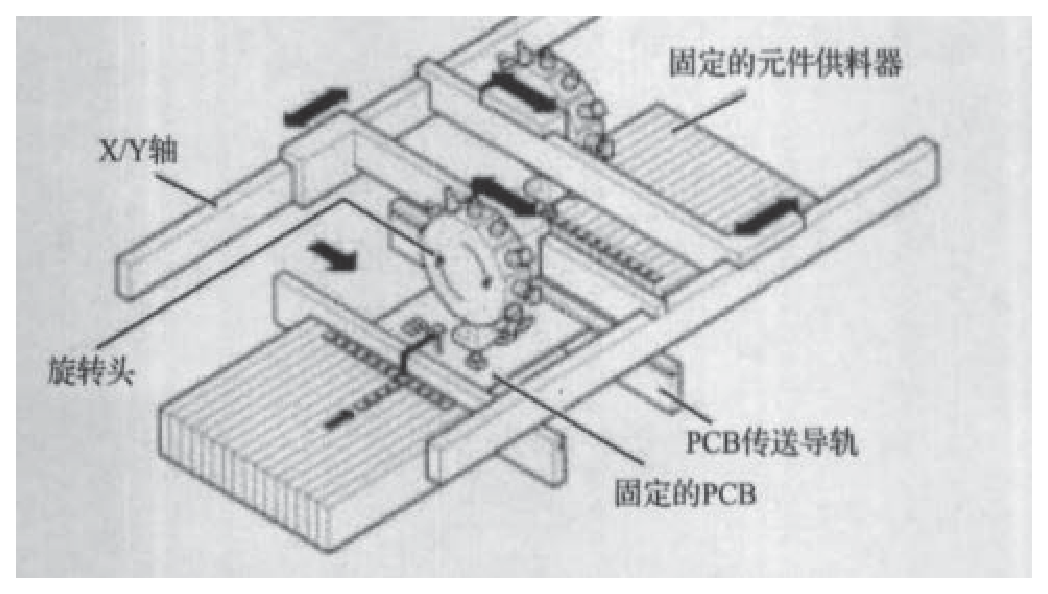
\includegraphics[width=0.6\textwidth]{fig302.eps}
\caption{双旋转头复合式机器结构图}
\label{fig302}
\end{figure}
\begin{figure}[htb!]
\centering
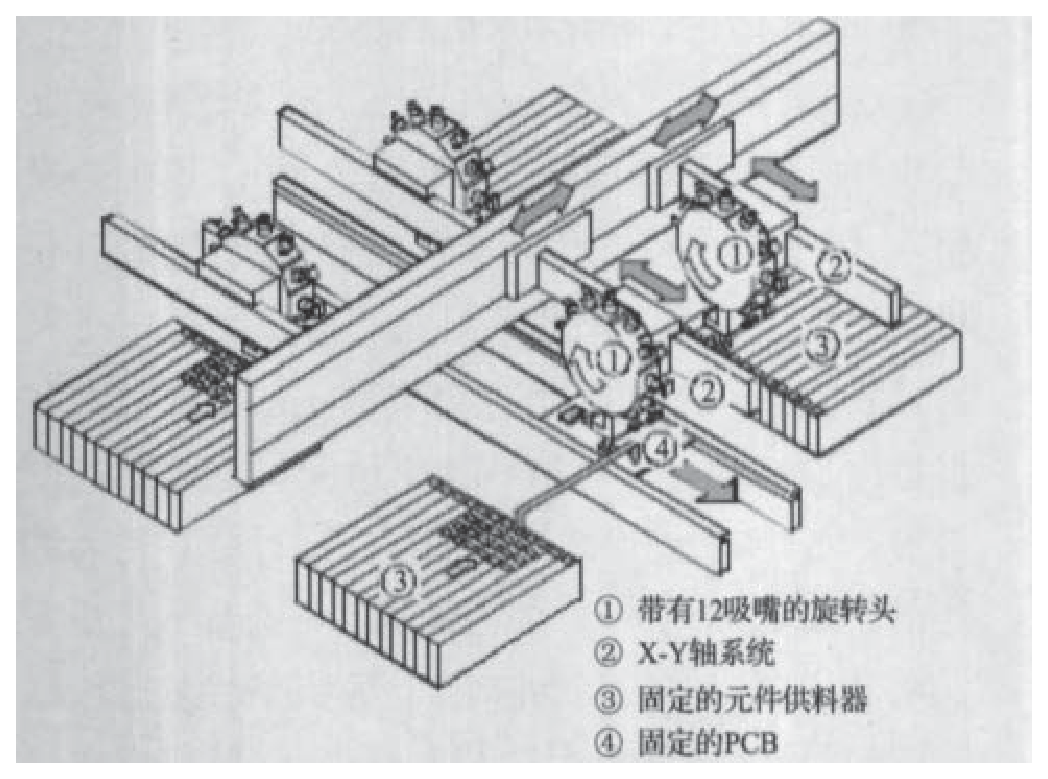
\includegraphics[width=0.6\textwidth]{fig303.eps}
\caption{四旋转头复合式机器结构图}
\label{fig303}
\end{figure}

\textbf{(3)转塔式}

砖塔的概念是使用一组移动的送料器,砖塔从这里吸取原件,然后把原件贴放在位于移动的工作台上的电路板上面,结构如图\ref{fig304}所示。转塔式机器由于拾取原件和贴装动作同时进行,使得贴片速度大幅度低声。这种结构的高速贴片机在我国的应用也很普遍,不但速度快,而且历经十余年的发展技术已经非常成熟,如Fuji公司的CP842E机器贴装速度可达到0.068s/片。但是这种机器由于机械结构所限,其贴装速度已达到一个极限值,不可能再大幅度提高。该机型的不足之处是只能处理带状料。

\begin{figure}[htb!]
\centering
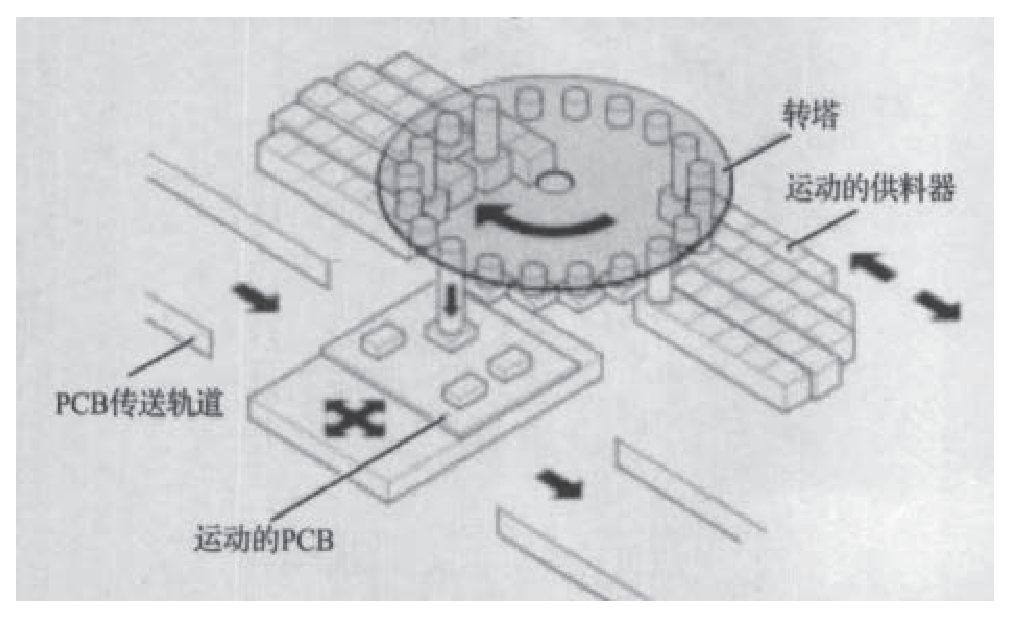
\includegraphics[width=0.6\textwidth]{fig304.eps}
\caption{转塔式机器结构图}
\label{fig304}
\end{figure}

转塔式机器主要应用于大规模的计算机办卡、移动电话、假单等产品的生产商,这是因为在这些产品当中个,阻容原件特别多、装配密度大、很适合采用这一机型进行生产。相当多的台资、港资组装企业已经国内电器生产商都蝉蛹这一机型,以满足高速组装的要求。生产转塔式机器的厂商主要有Panasonic、Hitachi和Fuji。

元件送料器放于一个单坐标移动的料车上,基板(PCB)放于一个X/Y坐标系统移动的工作台上,贴片头安装在一个转塔上,工作时,料车将元件送料器移动到取料位置,贴片头上的真空吸料嘴在取料位置取元件,经转塔转动到贴片位置(与取料位置成180度),在转动过程中经过对元件位置与方向的调整,将元件贴放于基板上。

对元件位置与方向的调整方法:

相机识别、X/Y坐标系统调整位置、吸嘴自旋转调整方向,相机固定,贴片头飞行划过相机上空,进行成像识别。

一般,转塔上安装有十几到二十几个贴片头,每个贴片头上安装2~4个真空吸嘴(较早机型)至5~6个真空吸嘴(现有机型)。由于转塔的特点,将动作细微化,选换吸嘴、送料器移动到位、取元件、元件识别、角度调整、工作台移动(包含位置调整)、贴放元件等动作都可以在同一时间周期内完成,所以实现真正意义上的高速度。目前最快的时间周期达到0.08~0.10秒钟一片元件。

此机型在速度上是优越的,适于大批量生产,但其只能用带状包装的元件,如果是密脚、大型的集成电路(IC),只有托盘包装,则无法完成,因此还有赖于其它机型来共同合作。这种设备结构复杂,造价昂贵,最新机型约在\$50万,是拱架型的三倍以上。

\textbf{(4)大型平行系统}

大规模平行系统(又称模组机)使用一系列小的单独的贴装单元(也称为模组)。每个单元有自己的丝杠位置系统,安装有相机和贴装头。每个贴装头可吸取有限的带式送料器,贴装PCB的一部分,PCB以固定的间隔时间在机器内步步推进。单独地各个单元机器运行速度较慢,可是他们连续或平行工作会得到很高的产量。如Assembleon公司的AX-5机器可最多有20个贴装头,实现了每小时15万片的贴装速度,堪称业界第一,但是就每个贴装头而言,贴装速度在每小时7500片左右,仍有大幅度提高的可能。这种机器也主要适用于规模化生产,例如手机和电脑主板等。生产大规模平行系统机器的厂商主要有Assembleon,Fuji公司也推出了采用类似结构的NXT型超高速贴片机、如图\ref{fig305}所示,通过搭载可以更换的贴装工作头,同一台机器既可以是高速机也可以是泛用机,几乎可以进行所有贴装元器件的贴装,从而使设备的初期投资及增加设备投资降低到最低程度。
\begin{figure}[htb!]
\centering
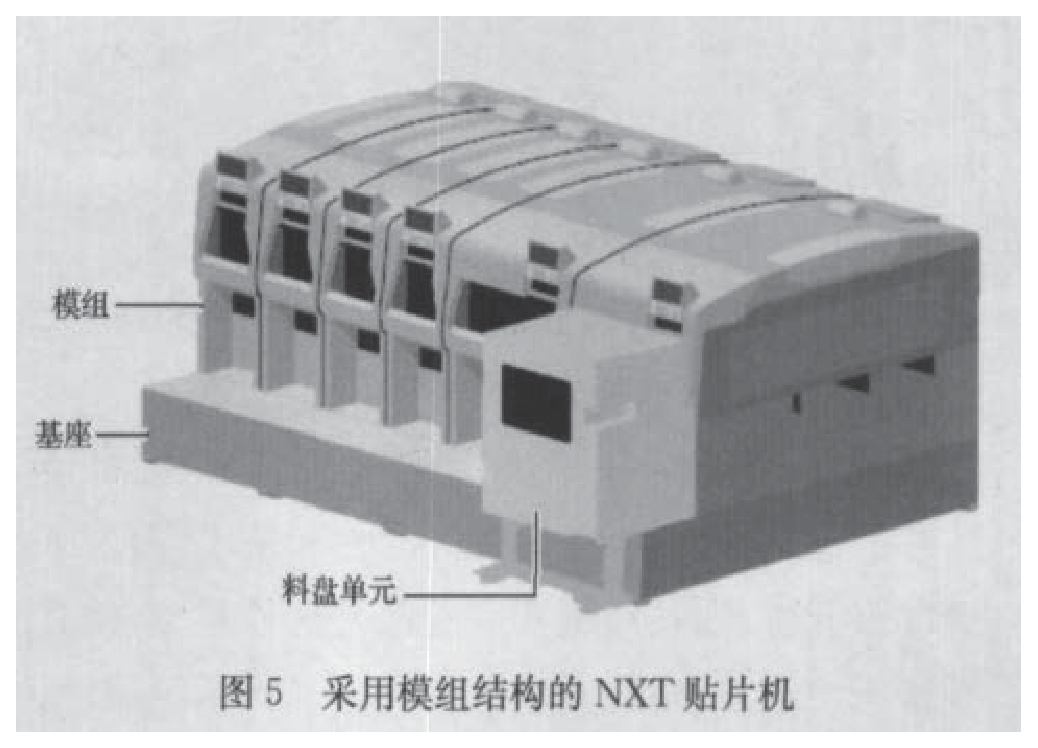
\includegraphics[width=0.6\textwidth]{fig305.eps}
\caption{大型平行系统结构图}
\label{fig305}
\end{figure}

\textbf{(5)柔性化的贴装方法}

上述的4中结构的设备都有着各自独特的特点和属性。许多公司使用两台平台以使其效率和性能达到最优化。最近五年来,愈来愈多的公司倾向于采用具有柔性功能的贴装设备,这种折衷的解决方案与常规的高精度模块相比较,综合了较高的贴装速度和大量的送料位置。这些平台依然能够满足绝大多数元器件全方位的贴装需求,可以从最小型的无源器件到最大型的有源器件。举例来说西门子公司推出的Siplace设备采用独特的柔性化手段,可以通过采集和贴装系统进行贴装,而垂直的旋转头系统能够用来拾取12个元器件。许多其他类型的拱架式、拾取和贴装设备使用多管路的工作头。同时的“群”拾取方式不能够很好地处理小型的元器件,因为他们在吸嘴与送料器之间要求极其精确地排列。在这些设备商极其精确是不可能办到的。可供选择的方法是单个地拾取原件,这样不可避免地使贴装所花费的时间大大地增加了。

展望未来,那种“柔性”的,多管路拱架式设备将成为小型至中型规模的定单型装配厂商所选择的设备。满足这个市场的理想设备是能够在高速状态下,具有从0201型器件至大型矩形扁平封装器件实现广泛贴装的能力。在这个局部市场上的竞争是相当激烈的,它能够使设备购买者在价格、效益和整个操作方面受益匪浅。而对大型电子装配厂商而言,具有多贴撞头构架的机器将大受欢迎,包括多臂式、复合式、大型平行系统等,这些机器也被称为模块机,由于可以根据未来需求灵活添加不同类型的贴装单元,满足未来柔性化生产的需求,当产品发生了变化以后,能够及时提升设备的工作适应能力是非常重要的,因为新的封装和电路板带来了新的要去。在一台贴装设备上进行投资往往应该基于现在的考虑和对未来的需求进行估计。购买一台比目前所需功能多得多的设备常常能够避免未来可能错失的商业机会。在现有设备上进行升级比购买一台新设备从经济上来说要合算得多。基于上述情况,很多高端贴片机设备厂商纷纷推出具有多贴装头的各种构架的机器,例如Universal的GC60、松下的CM602、日立的GHX-1、Siemens的HS60、Fuji的NXT等,并逐步取代转塔机器在高速机市场中的支配地位。
\subsubsection{工作头组件和轴结构}
工作头组件:在XY方向(或X方向)移动,从供料器中拾取零件和贴装在PCB上。

工作头组件移动手柄(Movement Handle):当伺服控制解除时,你可用手在每个方向移动,当用手移动工作头组件时通常用这个手柄。

X轴:移动工作头组件跟PCB传送方向平行。

Y轴:移动工作头组件跟PCB传送方向垂直。

Z轴:控制工作头组件的高度。

R轴:控制工作头组件吸嘴轴的旋转。

W轴:调整运输轨的宽度。
\subsubsection{运输轨部件}
传送组织是安放在导轨上的超薄型皮带传送体系,通常皮带安装在轨迹边际,其作用是将PCB 送到预订方位,贴片后再将其送至下一道工序。传送组织首要分为全体式和分段式两种,全体式方法下 PCB 的进入,贴片和送出一直在同一导轨上,选用限位块限位,定位销上行定位,压紧组织将PCB 压紧,支撑台板上支撑杆上移支撑来完结 PCB 的定位固定。定位销定位精度较低,需求高精度时也可选用光学体系,仅仅定位时刻较长。分段式 通常分为三段,前一段担任从上道技术接纳PCB,中心一端担任PCB定位压紧,后一段担任将PCB送至下一道工序,其长处是削减PCB传送时间。
运输轨部件包括:
1、主挡板(Main Stopper)

2、定位针 (Locate Pins)

3、Push-in Unit(入推部件)

4、边缘夹具 (Edge Clamp)

5、上推平板 (Push-up Plate)

6、上推顶针 (Push-up Pins)

7、入口挡板 (Entrance Stopper)
\subsubsection{吸嘴站}
吸嘴站(Nozzle Station):允许吸嘴的自动交换,总共可装载16个吸嘴,7个标准和9个可选吸嘴。
\subsubsection{气源部件}
包括空气过滤器、气压调节按钮、气压表。
\subsection{机电系统设计}
\subsection{图形图像算法}
高性能贴片机普遍采用视觉对中系统。视觉对中系统运用数字图像处理技术,当贴片头上的吸嘴吸取元件后,在移到贴片位置的过程中,由固定在贴片头上的或固定在机身某个位置上的照相机获取图像,并且通过影像探测元件的光密度分布,这些光密度以数字形式再经过照相机上许多细小精密的光敏元件组成的CCD光耦阵列,输出0~255级的灰度值。灰度值与光密度成正比,灰度值越大,则数字化图像越清晰。数字化信息经存储、编码、放大、整理和分析,将结果反馈到控制单元,并把处理结果输出到伺服系统中去调整补偿元件吸取的位置偏差,最后完成贴片操作。

视觉系统在成功的贴装设备中扮演着一个重要的角色。高精度的光学装置、灵活的照明和高解析度的工业相机集成出最佳的电路和器件的图像,并且通过现代化的算法能够获取至关重要的电路板、贴装元件及供料位置的修正信息。通过采用先进的视觉技术装置,能够达到较高水平的贴装速度,同时高精度的贴装位置,降低是去中所发生的缺陷、从而提高整条生产线上的上产量,增加经济效益。

视觉系统一般分为俯视,仰视、头部或者激光对准,视位置或者相机的类型而定。图\ref{fig3301}列出了一个典型的贴片视觉对中系统。
\begin{figure}[htb!]
\centering
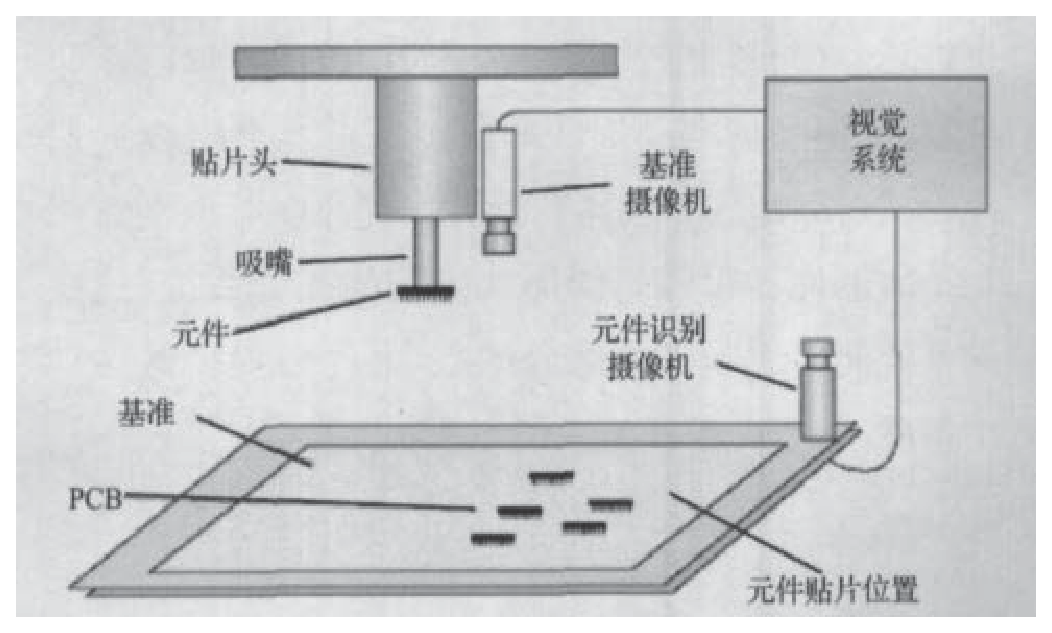
\includegraphics[width=0.6\textwidth]{fig3301.eps}
\caption{典型的贴片视觉对中系统}
\label{fig3301}
\end{figure}
\subsection{优化算法设计}
\section{泛用贴片机国内外现状}
\subsection{国外研究进展}
\subsection{国内研制情况}
\section{国产贴片机的瓶颈}
\section{我们的优势}
\section{展望}
国家意义重大;

系列机电产品,填补国家空白;

与国际垄断厂商抗衡;

技术有借鉴意义,可以移植;

吸引高技术人才;

上下游产业链形成;

\begin{table}[h]
\caption{地址 HT-03-04-02-10 对应数据}\label{HT-03-04-02-10}
\centering
\begin{tabular}{|c|c|c|c|}
相机类型数量 & 具体内容       & 地址                  & 数据  \\
飞行相机   & CCD面阵-6个     & HT-03-04-02-10-01    & 01-06   \\
上视相机   & CCD面阵-2个     & HT-03-04-02-10-02    & 01-02   \\
下视相机   & CCD面阵-1个     & HT-03-04-02-10-03    & 01-01
\end{tabular}
\end{table}


\bibliographystyle{IEEEtran}
\bibliography{reference}
\newpage
\end{CJK}
\end{document}

%This file should be compiled with latex!!!
